\section* {3.1}

\subsection{Постановка задачи}
Используя таблицу значений $Y_i$  функции $y=f(x)$, вычисленных в точках   $X_i, i=0,..3$  построить интерполяционные многочлены Лагранжа и Ньютона, проходящие через точки $\{X_i,Y_i \}$ .  Вычислить значение погрешности интерполяции в точке $X^*$. 

{\bfseries Вариант:} 10

$y=arctg(x), a)X_i= -3,-1,1,3;  б)X_i= -3,0,1,3;$
%\pagebreak

\subsection{Результаты работы}
\begin{figure}[h!]
\centering
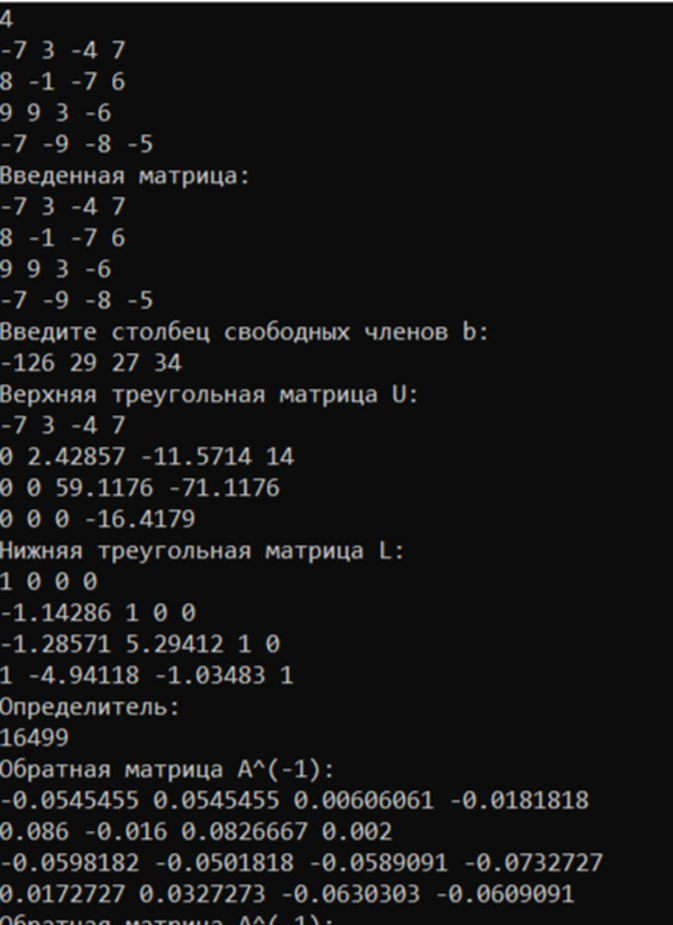
\includegraphics[width=12cm, height=3cm]{img}
\caption{Вывод программы в консоли}
\end{figure}
\pagebreak
% \vfill


\subsection{Исходный код}
% \lstinputlisting[language=C++]{matrix.cpp}
% \begin{lstlisting}
\lstinputlisting{include/3_1.cpp}
% \end{lstlisting}
% \lstinputlisting{matrix.cpp}
% {../../include/matrix.cpp}
% \pagebreak
% \lstinputlisting[title=\texttt{parabolic\_pde.hpp}]{../../include/partial_differential/parabolic_pde.hpp}
% \pagebreak
% 